\section{Cơ sở lý thuyết}

Chương này trình bày các nền tảng lý thuyết được sử dụng trong hệ thống SmartLock Fuzzy. Trọng tâm của hệ thống không phải là nhận diện khuôn mặt đơn lẻ, mà là chuỗi quyết định hoàn chỉnh gồm phát hiện khuôn mặt, nhận diện danh tính, đánh giá chất lượng ảnh, suy luận mờ mức rủi ro và điều khiển phần cứng khóa cửa. Vì vậy, các phần bên dưới được tổ chức theo đúng luồng xử lý của hệ thống hiện thực.

\subsection{Thị giác máy tính xử lý cục bộ}

Hệ thống xử lý ảnh trực tiếp trên Raspberry Pi thay vì gửi ảnh lên máy chủ bên ngoài. Cách tiếp cận này có ba lợi ích chính: giảm độ trễ, tránh phụ thuộc mạng và hạn chế việc truyền dữ liệu khuôn mặt ra khỏi thiết bị. Toàn bộ pipeline thị giác máy tính sử dụng OpenCV \cite{opencv}, gồm đọc frame từ camera, chuyển đổi màu, phát hiện khuôn mặt, nhận diện bằng mô hình LBPH và vẽ kết quả lên frame trả về frontend.

Camera trả về ảnh màu ở định dạng BGR. Tuy nhiên, Haar Cascade và LBPH đều làm việc hiệu quả trên ảnh grayscale, do đó frame được chuyển sang ảnh xám trước khi xử lý. Về mặt lý thuyết, một điểm ảnh màu $(R,G,B)$ có thể được chuyển thành độ sáng xấp xỉ theo công thức:

\begin{equation}
    Y = 0.299R + 0.587G + 0.114B
\end{equation}

Trong đó $Y$ là cường độ sáng của pixel trong ảnh grayscale. Ảnh xám giúp giảm số chiều dữ liệu từ ba kênh màu xuống một kênh, giảm chi phí tính toán và phù hợp với các đặc trưng hình học/kết cấu được dùng trong đề tài.

Trong hệ thống khóa cửa, yêu cầu quan trọng là phản hồi ổn định theo thời gian thực. Vì vậy, các thuật toán được chọn đều là thuật toán nhẹ, có thể chạy trên CPU của Raspberry Pi: Haar Cascade cho bước phát hiện và LBPH cho bước nhận diện. Các mô hình học sâu hiện đại có thể đạt độ chính xác cao hơn, nhưng thường cần GPU hoặc NPU để chạy mượt trong môi trường nhúng.

\subsection{Phát hiện khuôn mặt bằng Haar Cascade}

Haar Cascade là phương pháp phát hiện đối tượng cổ điển được đề xuất trong khung Viola--Jones \cite{viola2001}. Phương pháp này biểu diễn vùng ảnh bằng các đặc trưng Haar-like, tức là các hiệu giữa tổng cường độ sáng của những vùng chữ nhật sáng và tối. Với khuôn mặt người, một số tương phản thường gặp như vùng mắt tối hơn vùng má, sống mũi sáng hơn hai bên mặt, hoặc vùng miệng tạo ra các mẫu chữ nhật có khả năng phân biệt.

\subsubsection{Ảnh tích phân}

Để tính nhanh tổng cường độ trên nhiều vùng chữ nhật, Haar Cascade sử dụng ảnh tích phân. Với ảnh đầu vào $I(x,y)$, ảnh tích phân $S(x,y)$ được định nghĩa:

\begin{equation}
    S(x,y) = \sum_{i \le x,\ j \le y} I(i,j)
\end{equation}

Nhờ ảnh tích phân, tổng cường độ trong một vùng chữ nhật bất kỳ có thể tính bằng bốn phép truy cập thay vì cộng từng pixel. Điều này giúp bộ phát hiện quét nhiều vị trí và nhiều tỉ lệ khuôn mặt với tốc độ cao, phù hợp với xử lý video trực tiếp.

\subsubsection{Mô hình cascade}

Một frame camera có rất nhiều cửa sổ quét không chứa khuôn mặt. Cascade giải quyết vấn đề này bằng nhiều tầng phân loại nối tiếp. Các tầng đầu đơn giản, loại bỏ nhanh các vùng chắc chắn không phải khuôn mặt. Chỉ những vùng vượt qua tầng trước mới được đưa đến tầng sau phức tạp hơn. Nhờ đó, phần lớn chi phí tính toán chỉ tập trung vào các vùng có khả năng chứa khuôn mặt.

Trong đề tài, hệ thống dùng file cascade có sẵn \texttt{haarcascade\_frontalface\_default.xml} của OpenCV \cite{opencv}. Hàm \texttt{detectMultiScale} được gọi trên ảnh grayscale với các tham số chính như Bảng \ref{tab:haar_params}.

\begin{table}[H]
\centering
\caption{Các tham số chính của Haar Cascade trong hệ thống}
\label{tab:haar_params}
\begin{tabular}{|l|c|p{7.5cm}|}
\hline
\textbf{Tham số} & \textbf{Giá trị} & \textbf{Ý nghĩa} \\
\hline
\texttt{scaleFactor} & 1.1 & Mỗi lần quét, kích thước cửa sổ được thay đổi theo tỉ lệ 1.1 để phát hiện khuôn mặt ở nhiều khoảng cách khác nhau. \\
\hline
\texttt{minNeighbors} & 5 & Một vùng chỉ được chấp nhận nếu có đủ số cửa sổ lân cận cùng phát hiện, giúp giảm false positive. \\
\hline
\texttt{minSize} & $(30,30)$ & Loại bỏ các vùng quá nhỏ, thường là nhiễu hoặc khuôn mặt ở quá xa camera. \\
\hline
\end{tabular}
\end{table}

Nếu phát hiện nhiều khuôn mặt trong cùng một frame, hệ thống chỉ giữ khuôn mặt có diện tích bounding box lớn nhất. Quyết định này phù hợp với kịch bản khóa cửa, trong đó người đang xác thực thường đứng gần camera nhất. Các khuôn mặt nhỏ hơn ở nền sau không nên làm thay đổi quyết định mở khóa.

Ưu điểm của Haar Cascade là tốc độ nhanh, không cần GPU, dễ triển khai và đủ tốt khi người dùng nhìn tương đối thẳng vào camera. Hạn chế là độ chính xác giảm khi ánh sáng yếu, khuôn mặt quay nghiêng mạnh, bị che khuất hoặc góc đặt camera không ổn định. Vì vậy, hệ thống không dùng kết quả Haar một cách độc lập mà kết hợp thêm nhận diện LBPH và fuzzy logic để đánh giá rủi ro.


\begin{figure}[H]
    \centering
    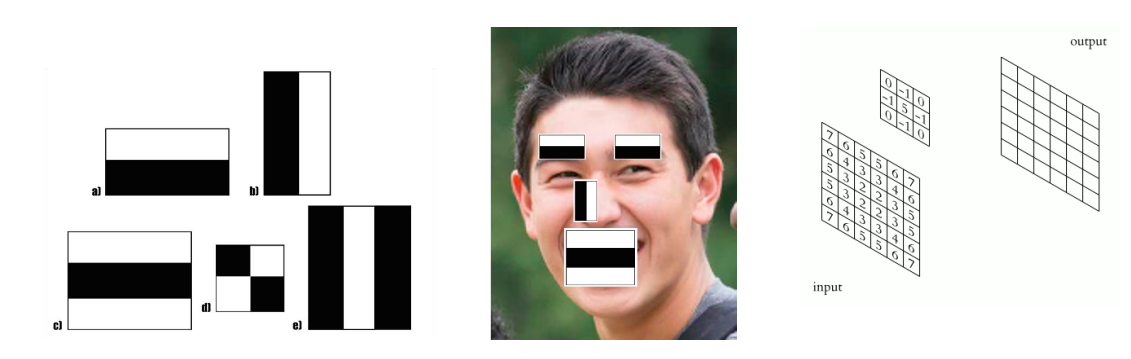
\includegraphics[width=1\linewidth]{haar_cascade.png}
    \caption{Minh họa kết quả phát hiện khuôn mặt bằng Haar Cascade}
    \label{fig:haar_detection}
\end{figure}
\subsection{Nhận diện khuôn mặt bằng LBPH}

LBPH (Local Binary Patterns Histograms) là phương pháp nhận diện khuôn mặt dựa trên mô tả kết cấu cục bộ \cite{lbph2006}. Thay vì học đặc trưng sâu, LBPH mã hóa mối quan hệ sáng/tối giữa một pixel trung tâm và các pixel lân cận. Điều này làm cho thuật toán nhẹ, dễ huấn luyện với số lượng mẫu nhỏ và phù hợp với thiết bị nhúng.

\subsubsection{Toán tử Local Binary Pattern}

Với một pixel trung tâm có cường độ $i_c$ và $P$ pixel lân cận có cường độ $i_p$, mã LBP được tính:

\begin{equation}
    LBP(x_c,y_c) = \sum_{p=0}^{P-1} s(i_p - i_c)2^p
\end{equation}

\begin{equation}
    s(u) =
    \begin{cases}
        1, & u \ge 0 \\
        0, & u < 0
    \end{cases}
\end{equation}

Kết quả là một số nhị phân mô tả mẫu kết cấu quanh pixel trung tâm. Ví dụ, vùng mắt, mũi, miệng và viền mặt tạo ra các mẫu sáng/tối khác nhau. Khi tính LBP cho toàn bộ ROI khuôn mặt, ta thu được bản đồ kết cấu cục bộ của khuôn mặt đó.

\subsubsection{Histogram theo lưới}

Nếu chỉ gom histogram trên toàn ảnh, thông tin vị trí của đặc trưng sẽ bị mất. Vì vậy LBPH chia khuôn mặt thành các ô lưới, tính histogram LBP cho từng ô, sau đó nối các histogram lại thành vector đặc trưng cuối cùng. Trong hệ thống, ROI khuôn mặt được resize về $100\times100$ pixel và mô hình LBPH được huấn luyện với các tham số ở Bảng \ref{tab:lbph_params}.

\begin{table}[H]
\centering
\caption{Tham số LBPH sử dụng khi huấn luyện}
\label{tab:lbph_params}
\begin{tabular}{|l|c|p{7.5cm}|}
\hline
\textbf{Tham số} & \textbf{Giá trị} & \textbf{Ý nghĩa} \\
\hline
\texttt{radius} & 1 & Bán kính vùng lân cận quanh pixel trung tâm. \\
\hline
\texttt{neighbors} & 8 & Số điểm lân cận dùng để tạo mã LBP. \\
\hline
\texttt{grid\_x} & 8 & Số ô chia theo chiều ngang khuôn mặt. \\
\hline
\texttt{grid\_y} & 8 & Số ô chia theo chiều dọc khuôn mặt. \\
\hline
Kích thước ROI & $100\times100$ & Kích thước chuẩn hóa trước khi huấn luyện và dự đoán. \\
\hline
\end{tabular}
\end{table}

Trong OpenCV, bộ nhận diện LBPH trả về hai giá trị \cite{opencv}:

\begin{itemize}
    \item \textbf{label}: mã định danh của người có histogram gần nhất với mẫu đầu vào.
    \item \textbf{confidence}: khoảng cách LBPH giữa mẫu đầu vào và mẫu đã học. Đây là khoảng cách, không phải xác suất; giá trị càng nhỏ thì khuôn mặt càng giống dữ liệu huấn luyện.
\end{itemize}

Hệ thống dùng ngưỡng \texttt{RECOGNITION\_THRESH = 150.0}. Nếu khoảng cách LBPH $d$ lớn hơn hoặc bằng ngưỡng này, khuôn mặt được xem là \texttt{Unknown}. Nếu nhỏ hơn ngưỡng, \texttt{label} được ánh xạ sang tên người dùng thông qua file JSON đi kèm mô hình.

\subsubsection{Chuẩn hóa độ tin cậy cho fuzzy logic}

Vì \texttt{confidence} của OpenCV LBPH là khoảng cách, hệ thống cần chuyển nó thành giá trị ``độ tin cậy mô hình'' theo hướng càng lớn càng đáng tin. Công thức được sử dụng:

\begin{equation}
    C_{raw} = \max\left(0,\ 100 - \frac{70d}{150}\right)
\end{equation}

Trong đó $d$ là khoảng cách LBPH. Khi $d=0$, mô hình có độ tin cậy rất cao. Khi $d=150$, giá trị còn khoảng 30, nằm gần vùng rủi ro cao trong bộ fuzzy. Trong bộ điều khiển fuzzy, biến \texttt{model\_confidence} được khai báo trên miền $[0,85]$; các giá trị cao hơn biên này được xem như mức HIGH tối đa.

\begin{figure}[H]
    \centering
    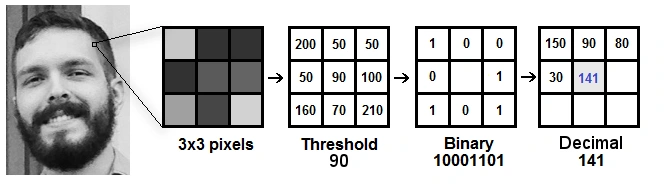
\includegraphics[width=1\linewidth]{lbph.png}
    \caption{Minh họa đặc trưng LBPH theo các vùng lưới của khuôn mặt}
    \label{fig:lbph_grid_todo}
\end{figure}

\subsection{Các đặc trưng chất lượng ảnh}

Kết quả nhận diện khuôn mặt phụ thuộc mạnh vào chất lượng ảnh. Một người đúng danh tính nhưng đứng trong ánh sáng quá yếu, quay mặt lệch hoặc frame bị mờ có thể làm tăng khoảng cách LBPH. Nếu hệ thống chỉ dùng ngưỡng nhận diện cứng, quyết định mở khóa có thể quá đơn giản. Vì vậy, hệ thống đo thêm ba đặc trưng chất lượng ảnh: độ sáng khuôn mặt, góc lệch tương đối và độ mờ.

\subsubsection{Độ sáng khuôn mặt}

Độ sáng được tính bằng giá trị trung bình của ảnh grayscale trong vùng khuôn mặt:

\begin{equation}
    I = \frac{1}{N}\sum_{p \in ROI} p
\end{equation}

Trong đó $ROI$ là vùng ảnh khuôn mặt và $N$ là số pixel trong vùng đó. Giá trị $I$ nằm trong khoảng $[0,255]$. Khi $I$ quá thấp, ảnh thiếu sáng và các chi tiết như mắt, mũi, miệng khó phân biệt. Khi $I$ quá cao, ảnh có thể bị cháy sáng, làm mất kết cấu cục bộ cần cho LBPH.

Trong bước đăng ký, hệ thống chỉ nhận mẫu nếu $35 \le I \le 230$. Khoảng này không đảm bảo ảnh hoàn hảo, nhưng loại bỏ được các frame quá tối hoặc quá sáng.

\subsubsection{Góc lệch tương đối}

Hệ thống không dùng mô hình head-pose estimation đầy đủ. Thay vào đó, góc lệch tương đối được ước lượng nhẹ bằng độ bất đối xứng sáng giữa nửa trái và nửa phải của ROI khuôn mặt:

\begin{equation}
    A = \frac{|\mu_L - \mu_R|}{\mu_L + \mu_R}
\end{equation}

\begin{equation}
    \theta = \min(180A,\ 90)
\end{equation}

Trong đó $\mu_L$ và $\mu_R$ là độ sáng trung bình của hai nửa khuôn mặt. Khi người dùng nhìn thẳng vào camera, hai nửa mặt thường có phân bố sáng tương đối cân bằng nên $A$ nhỏ. Khi mặt quay nghiêng hoặc một nửa mặt bị tối mạnh, $A$ tăng và góc ước lượng $\theta$ lớn hơn.

Cách ước lượng này có chi phí thấp và đủ dùng như một tín hiệu chất lượng cho fuzzy logic. Tuy nhiên, nó không phải là góc yaw hình học chính xác. Các trường hợp ánh sáng chiếu lệch mạnh có thể làm hệ thống đánh giá mặt đang bị lệch dù người dùng vẫn nhìn thẳng.

\subsubsection{Độ mờ khi đăng ký}

Khi đăng ký khuôn mặt, hệ thống dùng phương sai Laplacian để loại ảnh mờ. Laplacian phản ứng mạnh với biên và chi tiết cao tần. Nếu ảnh bị mờ, biên yếu đi và phương sai Laplacian giảm:

\begin{equation}
    B = Var(\nabla^2 ROI)
\end{equation}

Nếu $B < 20$, frame bị xem là quá mờ và không được lưu làm mẫu huấn luyện. Việc lọc mẫu mờ trong giai đoạn đăng ký rất quan trọng, vì dữ liệu đăng ký kém sẽ làm LBPH học histogram không đại diện, từ đó tăng lỗi nhận diện trong giai đoạn vận hành.

\begin{table}[H]
\centering
\caption{Điều kiện lọc mẫu khi đăng ký khuôn mặt}
\label{tab:registration_quality}
\begin{tabular}{|l|c|p{7cm}|}
\hline
\textbf{Tiêu chí} & \textbf{Ngưỡng} & \textbf{Mục đích} \\
\hline
Số khuôn mặt & Đúng 1 & Tránh gán nhầm mẫu của người khác vào identity đang đăng ký. \\
\hline
Kích thước mặt & $\min(w,h) \ge 32$ & Loại khuôn mặt quá nhỏ hoặc đứng quá xa camera. \\
\hline
Độ sáng & $35 \le I \le 230$ & Loại frame quá tối hoặc quá sáng. \\
\hline
Góc lệch & $\theta \le 40^\circ$ & Ưu tiên mẫu nhìn tương đối thẳng vào camera. \\
\hline
Độ mờ & $B \ge 20$ & Loại frame nhòe, rung hoặc mất chi tiết. \\
\hline
Khoảng cách thời gian & $\ge 0.25$s & Tránh lưu quá nhiều frame gần như giống hệt nhau. \\
\hline
Khác biệt với mẫu trước & $\ge 1.5$ & Khuyến khích người dùng thay đổi nhẹ tư thế để tăng đa dạng dữ liệu. \\
\hline
\end{tabular}
\end{table}

Sau khi một mẫu được chấp nhận, ROI được resize về $100\times100$ và cân bằng histogram bằng \texttt{equalizeHist}. Bước cân bằng histogram giúp giảm ảnh hưởng của chênh lệch sáng nhẹ giữa các lần chụp.

\subsection{Fuzzy logic Mamdani}

Fuzzy logic cho phép biểu diễn các khái niệm không có ranh giới cứng như ``độ tin cậy cao'', ``ánh sáng bình thường'' hoặc ``góc mặt lệch'' \cite{zadeh1965}. Trong khóa cửa thông minh, cách tiếp cận này phù hợp hơn một luật ngưỡng đơn giản vì quyết định truy cập nên xét đồng thời nhiều yếu tố. Ví dụ, một khuôn mặt có LBPH tốt nhưng ánh sáng quá xấu có thể cần rủi ro trung bình thay vì mở khóa ngay.

Hệ thống sử dụng bộ suy luận Mamdani \cite{mamdani1975} được hiện thực bằng pyfuzzylite \cite{fuzzylite}. Bộ điều khiển gồm bốn bước:

\begin{enumerate}
    \item \textbf{Fuzzification}: chuyển giá trị số thành mức thuộc về các tập mờ.
    \item \textbf{Rule evaluation}: đánh giá các luật IF--THEN bằng toán tử mờ.
    \item \textbf{Aggregation}: gom kết quả của nhiều luật thành một tập mờ đầu ra.
    \item \textbf{Defuzzification}: chuyển tập mờ đầu ra thành một giá trị rủi ro cụ thể.
\end{enumerate}

\subsubsection{Hàm thành viên Gaussian}

Các tập mờ trong hệ thống dùng hàm thành viên Gaussian:

\begin{equation}
    \mu(x) = \exp\left(-\frac{(x-c)^2}{2\sigma^2}\right)
\end{equation}

Trong đó $c$ là tâm của tập mờ và $\sigma$ là độ lệch chuẩn. Hàm Gaussian tạo ra biên chuyển mềm giữa các mức LOW, MEDIUM, HIGH thay vì thay đổi đột ngột tại một ngưỡng duy nhất.

\begin{table}[H]
\centering
\caption{Biến đầu vào của bộ fuzzy}
\label{tab:fuzzy_inputs}
\begin{tabular}{|l|c|l|}
\hline
\textbf{Biến} & \textbf{Miền giá trị} & \textbf{Tập mờ Gaussian $(c,\sigma)$} \\
\hline
Độ tin cậy mô hình & 0--85 & LOW $(0,17)$, MEDIUM $(42.5,10)$, HIGH $(85,17)$ \\
\hline
Độ sáng khuôn mặt & 0--255 & DARK $(0,40)$, NORMAL $(128,45)$, BRIGHT $(255,40)$ \\
\hline
Góc lệch khuôn mặt & 0--90 & FRONTAL $(0,20)$, MARGINAL $(90,40)$ \\
\hline
\end{tabular}
\end{table}

Biến đầu ra là \textbf{security risk} trong khoảng $[0,1]$. Giá trị càng gần 0 thì hệ thống càng an toàn để mở khóa; giá trị càng gần 1 thì rủi ro càng cao.

\begin{table}[H]
\centering
\caption{Biến đầu ra của bộ fuzzy}
\label{tab:fuzzy_output}
\begin{tabular}{|l|c|l|}
\hline
\textbf{Biến} & \textbf{Miền giá trị} & \textbf{Tập mờ Gaussian $(c,\sigma)$} \\
\hline
Security risk & 0--1 & MINIMUM $(0,0.1)$, AVERAGE $(0.5,0.1)$, MAXIMUM $(1,0.08)$ \\
\hline
\end{tabular}
\end{table}

Các hàm thành viên trong Bảng \ref{tab:fuzzy_inputs} và Bảng \ref{tab:fuzzy_output} được minh họa ở Hình \ref{fig:fuzzy_membership_todo}. Phần giao nhau giữa các đường cong cho phép một frame kích hoạt đồng thời nhiều luật với các mức độ khác nhau, nhờ đó quyết định không bị phụ thuộc vào một ngưỡng cứng duy nhất.

\begin{figure}[H]
    \centering
    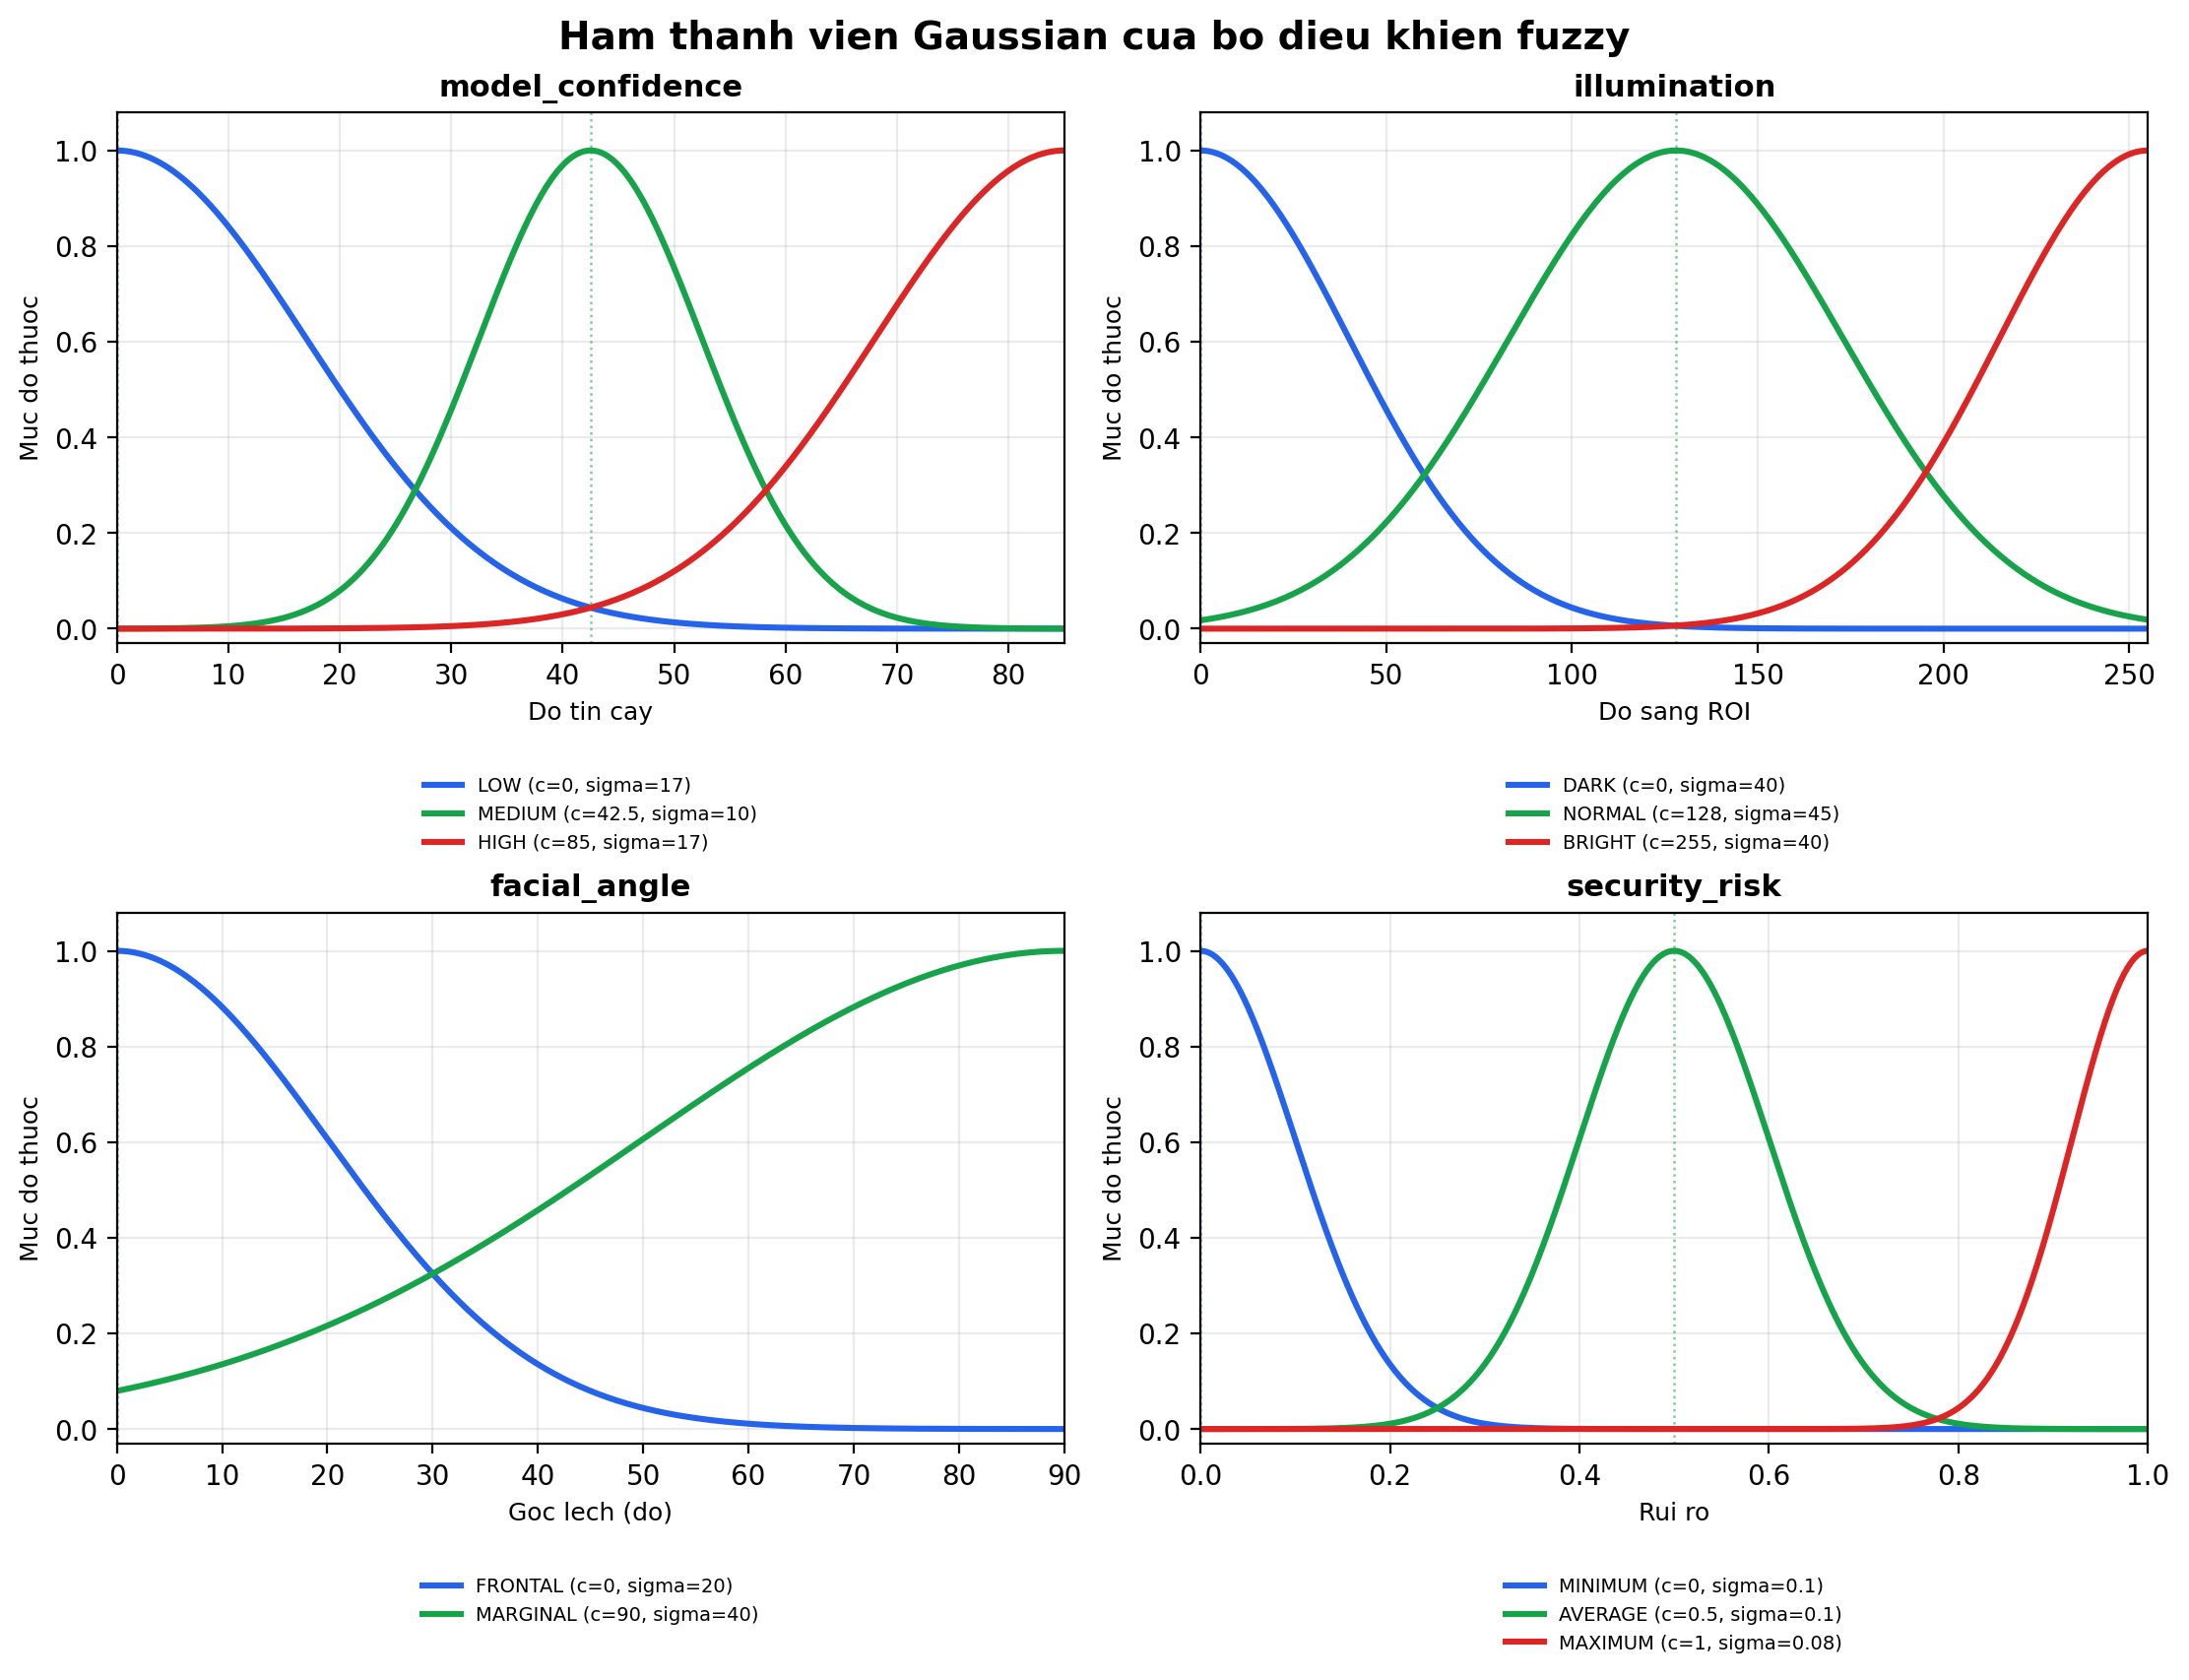
\includegraphics[width=\linewidth]{fuzzy_full.png}
    \caption{Minh họa các hàm thành viên của bộ điều khiển fuzzy}
    \label{fig:fuzzy_membership_todo}
\end{figure}

\subsubsection{Toán tử Mamdani và giải mờ}

Trong bộ điều khiển, phép AND được cài bằng toán tử Minimum, phép OR bằng Maximum, phép suy diễn bằng Minimum và phép tổng hợp các luật bằng Maximum. Sau khi tổng hợp, hệ thống dùng phương pháp centroid để giải mờ:

\begin{equation}
    r = \frac{\int z\mu_{out}(z)\,dz}{\int \mu_{out}(z)\,dz}
\end{equation}

Trong đó $r$ là giá trị rủi ro rõ cuối cùng, còn $\mu_{out}(z)$ là hàm thành viên đầu ra sau khi tất cả luật được kích hoạt. Trong code, centroid được lấy mẫu với độ phân giải 200 điểm, đủ cho miền đầu ra nhỏ $[0,1]$.

\subsubsection{Nhóm luật quyết định}

Bộ điều khiển sử dụng 13 luật. Các luật được thiết kế theo nguyên tắc fail-safe: khi danh tính không đáng tin hoặc điều kiện ảnh xấu, rủi ro phải tăng; hệ thống chỉ mở khóa khi độ tin cậy cao, ánh sáng bình thường và khuôn mặt nhìn thẳng.

\begin{table}[H]
\centering
\caption{Tóm tắt nhóm luật fuzzy}
\label{tab:fuzzy_rule_groups}
\begin{tabular}{|p{3.2cm}|p{3.4cm}|p{2.8cm}|p{2.5cm}|}
\hline
\textbf{Model confidence} & \textbf{Illumination} & \textbf{Facial angle} & \textbf{Risk} \\
\hline
LOW & Bất kỳ & Bất kỳ & MAXIMUM \\
\hline
HIGH & NORMAL & FRONTAL & MINIMUM \\
\hline
HIGH & NORMAL & MARGINAL & AVERAGE \\
\hline
HIGH & DARK hoặc BRIGHT & Bất kỳ & AVERAGE \\
\hline
MEDIUM & NORMAL & FRONTAL & AVERAGE \\
\hline
MEDIUM & NORMAL & MARGINAL & MAXIMUM \\
\hline
MEDIUM & DARK & Bất kỳ & MAXIMUM \\
\hline
MEDIUM & BRIGHT & FRONTAL hoặc MARGINAL & AVERAGE \\
\hline
\end{tabular}
\end{table}

Nếu không có khuôn mặt trong frame, hệ thống không chạy mở khóa mà trả về rủi ro 1.0 và hành động \texttt{deny}. Nếu thư viện pyfuzzylite không khả dụng, backend có fallback logic tĩnh để hệ thống vẫn chạy theo hướng an toàn: độ tin cậy thấp hoặc điều kiện ảnh kém luôn dẫn tới rủi ro cao.

\subsubsection{Ánh xạ rủi ro thành hành động}

Giá trị crisp cuối cùng được ánh xạ thành hành động như Bảng \ref{tab:risk_action_map}. Hành động \texttt{otp} được hiểu là trạng thái cần xác thực bổ sung; trong bản hiện thực hiện tại, luồng keypad đóng vai trò kênh xác thực thứ hai độc lập.

\begin{table}[H]
\centering
\caption{Ánh xạ rủi ro thành hành động}
\label{tab:risk_action_map}
\begin{tabular}{|c|l|l|}
\hline
\textbf{Khoảng rủi ro} & \textbf{Hành động} & \textbf{Ý nghĩa} \\
\hline
$r < 0.30$ & \texttt{unlock} & Mở khóa bằng servo. \\
\hline
$0.30 \le r < 0.60$ & \texttt{otp} & Cần xác thực bổ sung. \\
\hline
$0.60 \le r < 0.85$ & \texttt{deny} & Từ chối truy cập và ghi nhận sự kiện. \\
\hline
$r \ge 0.85$ & \texttt{lockout} & Rủi ro rất cao, khóa tạm thời hoặc cảnh báo. \\
\hline
\end{tabular}
\end{table}

\subsection{Xác thực bằng keypad và mã PIN}

Ngoài nhận diện khuôn mặt, hệ thống có keypad 4x4 để nhập mã PIN 6 chữ số. Đây là một kênh xác thực khác với nhận diện khuôn mặt, giúp người dùng vẫn có thể mở khóa trong trường hợp camera, ánh sáng hoặc mô hình nhận diện không hoạt động tốt.

Về mặt bảo mật, hệ thống không so sánh trực tiếp chuỗi PIN dạng rõ. PIN được băm bằng SHA-256:

\begin{equation}
    H = SHA256(PIN)
\end{equation}

Khi người dùng nhập PIN, hệ thống băm chuỗi vừa nhập và so sánh với hash đang lưu trong bộ nhớ. Hàm băm một chiều giúp tránh việc lưu trực tiếp mật khẩu dạng rõ trong biến trạng thái. Mã PIN mới cũng phải có đúng 6 chữ số và chỉ được cập nhật khi người dùng nhập đúng PIN hiện tại.

Để hạn chế thử sai liên tục, keypad dùng cơ chế lockout. Sau 5 lần nhập sai, keypad bị khóa trong 30 giây. Ngoài ra, nếu người dùng bắt đầu nhập nhưng dừng quá lâu, buffer nhập PIN được xóa sau 10 giây. Các cơ chế này làm giảm nguy cơ brute-force đơn giản trên keypad vật lý.

\subsection{FastAPI, REST và cơ chế polling}

FastAPI là framework Python dùng để xây dựng API bất đồng bộ, có kiểu dữ liệu rõ ràng và tự sinh tài liệu OpenAPI \cite{fastapi}. Trong hệ thống, FastAPI quản lý vòng đời backend, khởi động camera worker khi ứng dụng start và dừng worker khi shutdown. Backend cũng cung cấp các endpoint để frontend đọc frame mới nhất, xem trạng thái camera, đăng ký khuôn mặt và đổi mật khẩu keypad.

Luồng camera không được truyền bằng WebSocket hay RTSP. Thay vào đó, worker xử lý frame trong background thread, encode frame đã vẽ kết quả thành JPEG base64 và lưu vào cache mới nhất. Frontend gọi \texttt{/api/v1/camera/frame} theo chu kỳ ngắn để lấy frame và metadata. Cơ chế này gọi là polling.

\begin{table}[H]
\centering
\caption{Các endpoint REST chính liên quan đến cơ sở lý thuyết hệ thống}
\label{tab:rest_theory_endpoints}
\begin{tabular}{|l|l|p{6.2cm}|}
\hline
\textbf{Phương thức} & \textbf{Endpoint} & \textbf{Vai trò} \\
\hline
GET & \texttt{/api/v1/camera/frame} & Trả về frame JPEG base64, danh sách khuôn mặt, kết quả fuzzy và trạng thái đăng ký. \\
\hline
GET & \texttt{/api/v1/camera/history} & Trả về lịch sử gần đây của nhận diện và quyết định truy cập. \\
\hline
POST & \texttt{/api/v1/register/start} & Bắt đầu phiên thu mẫu khuôn mặt cho một người dùng. \\
\hline
POST & \texttt{/api/v1/register/cancel} & Hủy phiên đăng ký đang chạy. \\
\hline
POST & \texttt{/api/v1/keypad/password} & Đổi mã PIN keypad sau khi xác thực PIN hiện tại. \\
\hline
GET & \texttt{/api/v1/keypad/status} & Trả về trạng thái keypad, số lần sai và thời gian lockout còn lại. \\
\hline
\end{tabular}
\end{table}

Polling có ưu điểm là đơn giản, dễ debug, dễ triển khai trong demo cục bộ và tương thích tốt với HTTP thông thường. Nhược điểm là frontend vẫn gửi request định kỳ kể cả khi frame không đổi. Trong hệ thống này, chu kỳ polling khoảng 250 ms là phù hợp vì frame đã được xử lý ở backend và kích thước ảnh JPEG base64 không quá lớn.

\subsection{Frontend Next.js}

Next.js là framework React hỗ trợ xây dựng giao diện web hiện đại \cite{nextjs}. Frontend trong đề tài đóng vai trò dashboard quan sát và điều khiển. Nó không truy cập camera trực tiếp, không chạy mô hình nhận diện và không điều khiển GPIO. Tất cả thao tác phần cứng và xử lý ảnh nằm ở backend; frontend chỉ gửi HTTP request và hiển thị dữ liệu nhận được.

Component hiển thị video gọi API theo chu kỳ, nhận \texttt{frame\_base64}, chuyển thành URL dạng \texttt{data:image/jpeg;base64,...} và hiển thị bằng thẻ \texttt{img}. Cùng với ảnh, frontend hiển thị số khuôn mặt, danh tính, khoảng cách LBPH, độ sáng, góc mặt, hành động fuzzy và phần trăm rủi ro. Cách hiển thị này giúp người vận hành quan sát được không chỉ kết quả cuối cùng, mà cả lý do hệ thống đưa ra quyết định.

Frontend cũng cung cấp form đăng ký khuôn mặt và form đổi mật khẩu keypad. Các form này kiểm tra dữ liệu cơ bản ở phía trình duyệt, ví dụ mã PIN phải gồm đúng 6 chữ số, sau đó gửi request đến FastAPI để xử lý chính thức.

\subsection{Nền tảng Raspberry Pi và ngoại vi}

Raspberry Pi đóng vai trò bộ điều khiển trung tâm của hệ thống \cite{raspberrypi}. Thiết bị vừa chạy backend Python, vừa đọc camera, vừa giao tiếp với keypad, OLED và servo. Các ngoại vi này giúp hệ thống hoạt động như một khóa cửa vật lý thay vì chỉ là demo nhận diện trên màn hình.

\subsubsection{Keypad ma trận 4x4}

Keypad 4x4 gồm 4 hàng và 4 cột. Về nguyên lý, mỗi phím là một công tắc nối một hàng với một cột. Để xác định phím được nhấn, hệ thống đặt các chân hàng làm output và các chân cột làm input với pull-down. Khi có cạnh rising ở một cột, callback ngắt được kích hoạt. Sau đó backend lần lượt kéo từng hàng lên mức HIGH để tìm giao điểm hàng--cột tương ứng với phím.

Cách dùng interrupt giúp giảm tải CPU so với việc polling keypad liên tục. Hệ thống cũng áp dụng debounce 250 ms để giảm hiện tượng một lần nhấn phím bị ghi nhận thành nhiều lần do rung tiếp điểm cơ khí.

\subsubsection{OLED SSD1306}

OLED SSD1306 kích thước 128x64 được dùng để hiển thị trạng thái hệ thống: màn hình chờ, nhập PIN, đăng ký khuôn mặt, mở khóa thành công, từ chối truy cập và lockout. Thư viện luma.oled được sử dụng để giao tiếp với màn hình \cite{lumaoled}. Backend render nội dung bằng Pillow rồi gửi buffer ảnh sang OLED qua bus SPI.

OLED rất quan trọng trong kịch bản khóa cửa vì người dùng đứng trước cửa không nhất thiết đang nhìn dashboard web. Các thông báo như số chữ số PIN đã nhập, số lần sai còn lại hoặc thời gian lockout cần được hiển thị trực tiếp trên thiết bị.

\subsubsection{Servo điều khiển chốt khóa}

Servo mô phỏng cơ cấu chốt khóa cửa. Servo được điều khiển bằng PWM 50 Hz. Trong hệ thống, duty cycle khoảng 7.5 dùng cho trạng thái mở khóa và khoảng 2.5 dùng cho trạng thái khóa. Sau khi servo quay đến vị trí mong muốn, duty cycle được đưa về 0 để giảm rung, giảm tiếng kêu và tiết kiệm năng lượng.

Servo nên dùng nguồn 5V ngoài thay vì lấy trực tiếp từ chân 5V của Raspberry Pi. Dòng khởi động của servo có thể làm sụt áp và khiến Pi reset. Tuy nhiên, nguồn servo và Raspberry Pi phải nối chung GND để tín hiệu PWM có cùng mức tham chiếu.

\begin{table}[H]
\centering
\caption{Các ngoại vi chính của hệ thống}
\label{tab:hardware_theory}
\begin{tabular}{|l|l|p{6.7cm}|}
\hline
\textbf{Thiết bị} & \textbf{Giao tiếp} & \textbf{Vai trò} \\
\hline
Camera USB/V4L2 & Video capture & Cung cấp frame đầu vào cho pipeline Haar, LBPH và fuzzy. \\
\hline
Keypad 4x4 & GPIO input/output & Nhập mã PIN 6 chữ số và xác thực dự phòng. \\
\hline
OLED SSD1306 & SPI & Hiển thị trạng thái trực tiếp trên thiết bị. \\
\hline
Servo & PWM 50 Hz & Mô phỏng cơ cấu mở/khóa chốt cửa. \\
\hline
\end{tabular}
\end{table}
